\newcommand{\FigTheoryMuonDecayCloudChamber}{
\begin{figure}[tb]
\centering 
%\fbox{
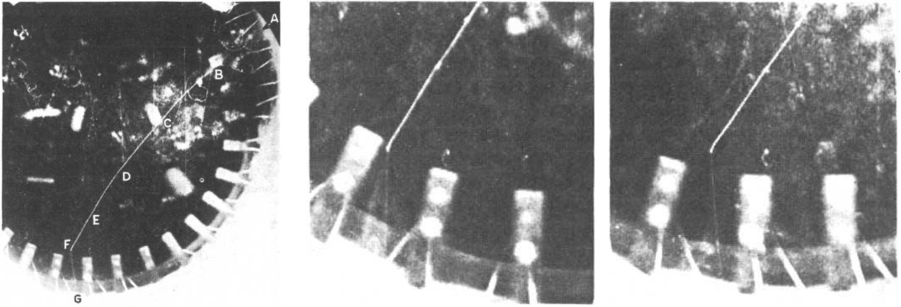
\includegraphics[width=0.95\textwidth]{figs/theory/EarlyCloudChamberMuonDecay.pdf}
%}
\caption{\figlabel{theory:muonCloudChamber}
One of the earliest cloud chamber photographs of a muon, taken in 1940~\cite{Williams1940102}.
In the left-most image the muon enters the chamber at point A and travels to point F, where it eventually decays to an electron which can be seen faintly leaving the image at point G.
The images to the right are a stereoscopic zoom in on point F, showing the relatively slow and more ionising muon and the faster, less ionising electron.
}
%\footnote{though the author has failed to reproduce the stereoscopic effect with his own eyes}
\end{figure}
}

\newcommand{\FigTheoryHincksPontecorvoMuEGamma}{
\begin{figure}[tb]
\centering 
%\fbox{
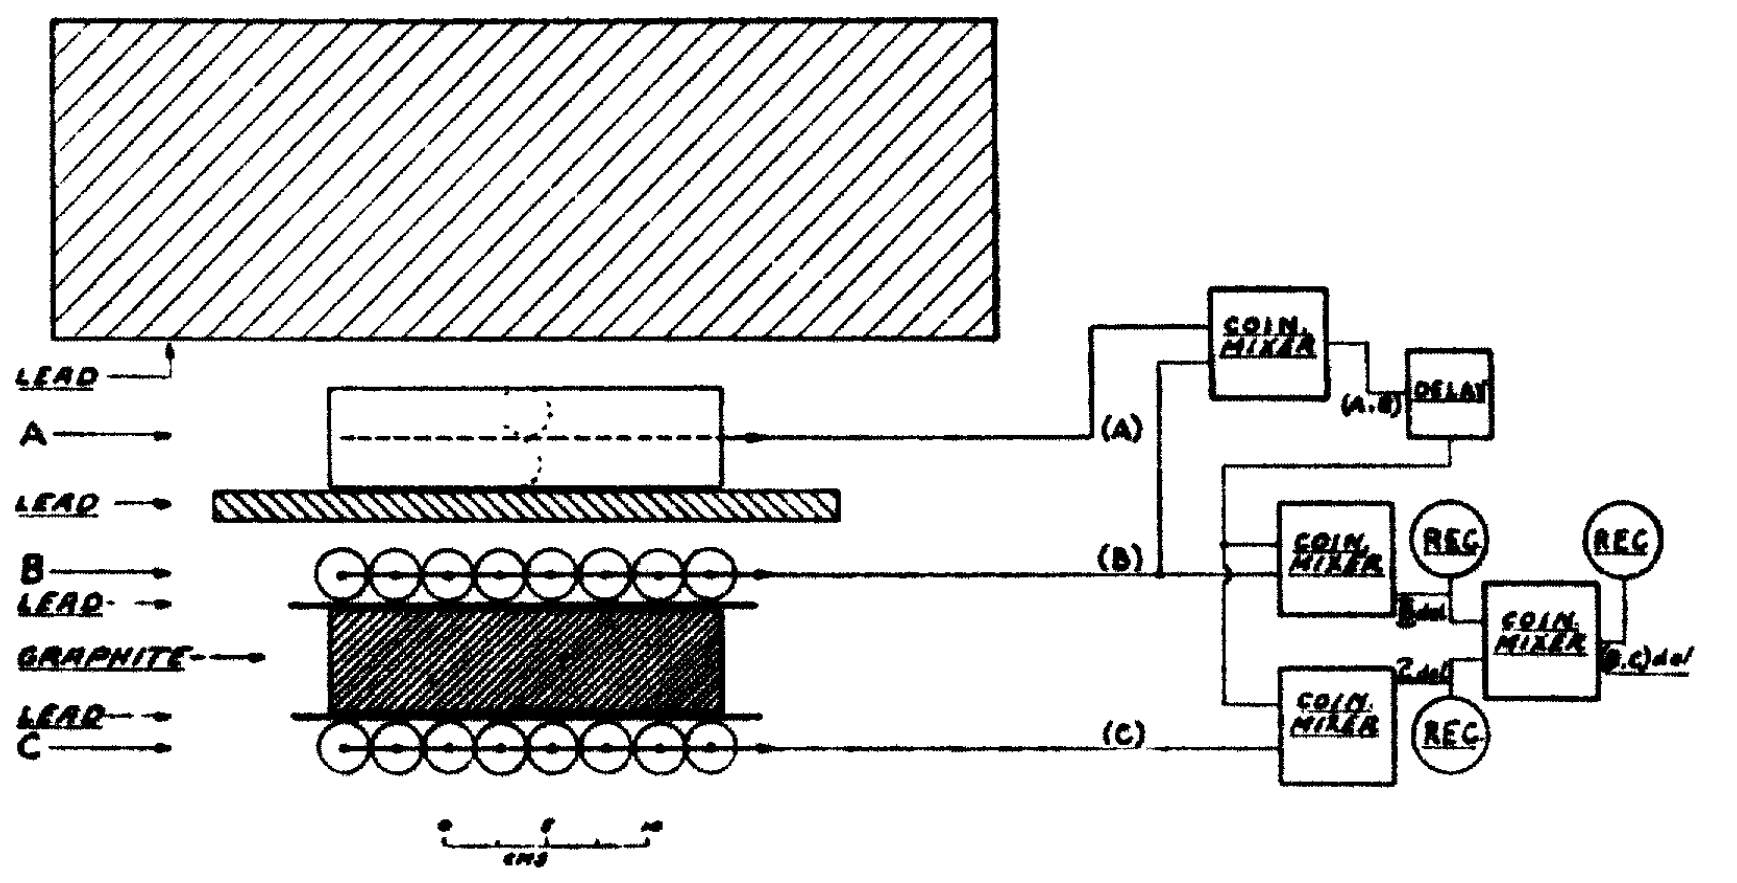
\includegraphics[width=0.85\textwidth]{figs/theory/OriginalMuEGammaExperiment.png}
%}
\caption{\figlabel{theory:originalMEG}
The setup of the first experiment to look for photons produced during muon decay taken from~\cite{Hincks194802}.
Cosmic muons arrived from the top, slowing down in the big block of lead, triggering two Geiger-Muller counters (A and B) as they passed and eventually coming to stop in the graphite.
From there, electrons and any potential photons would be detected in the counters above and below the graphite (B and C).  
No photons were seen in coincidence with an electron from muon decay, which lead theorists to hypothesise two distinct neutrino flavours.
}
%\footnote{though the author has failed to reproduce the stereoscopic effect with his own eyes}
\end{figure}
}

\newcommand{\FigTheoryMuEGammViaNeutrino}{
\begin{figure}[bt]
\centering 
%\fbox{
%\input{figs/feynman/mu_to_e_gamma_via_SM-Wgamma.tex}
\subfloat[][\figlabel{theory:feyn:muDecay}\ac{SM} Muon Decay]{\includegraphics[width=0.45\textwidth]{figs/feynman/pdfs/mu_decay.pdf}}\hspace{0.03\textwidth}
\subfloat[][\figlabel{theory:feyn:muEGammaViaNu}Neutrinoless Muon Decay with Photon Emission]{\includegraphics[width=0.45\textwidth]{figs/feynman/pdfs/mu_to_e_gamma_via_SM-Wgamma.pdf}}
%}
\caption{\figlabel{theory:feyn:decay}
Feynman diagram for the neutrinoless muon decay to a photon and electron mediated by a neutrino oscillation.
Although allowed in the \ac{SM} with neutrino oscillations, the actual rate from this diagram is well below present experiment sensitivities.
A similar diagram was envisaged to show that the lack of observation of \mueg implied distinict neutrino flavours.
}
%\footnote{though the author has failed to reproduce the stereoscopic effect with his own eyes}
\end{figure}
}

\newcommand{\FigTheoryMuEConvViaNeutrino}{
\begin{figure}[b]
\centering 
%\fbox{
%\input{figs/feynman/mu_to_e_gamma_via_SM-Wgamma.tex}
\subfloat[][\figlabel{theory:feyn:muecViaNu:W}$\gamma$ Penguin]  {\includegraphics[width=0.43\textwidth]{figs/feynman/pdfs/mu_e_conversion_via_SM-Wgamma.pdf}}\hspace{0.08\textwidth}
\subfloat[][\figlabel{theory:feyn:muecViaNu:Z}$Z$ Penguin]  {\includegraphics[width=0.43\textwidth]{figs/feynman/pdfs/mu_e_conversion_via_SM-nuZ.pdf}}\\
\subfloat[][\figlabel{theory:feyn:muecViaNu:d}$d$-quark Box]{\includegraphics[width=0.43\textwidth]{figs/feynman/pdfs/mu_e_conversion_via_SM-downBox.pdf}}\hspace{0.08\textwidth}
\subfloat[][\figlabel{theory:feyn:muecViaNu:u}$u$-quark Box]{\includegraphics[width=0.43\textwidth]{figs/feynman/pdfs/mu_e_conversion_via_SM-upBox.pdf}}\\
%}
\caption{\figlabel{theory:feyn:muecViaNu}
Feynman diagram for the neutrinoless muon decay in the presence of an atomic nucleus -- \mueconv{} -- caused by neutrino oscillations.
Compared to \mueg there are now four possible diagrams, so that the rate depends on the nucleus and picks up interference terms.
}
%\footnote{though the author has failed to reproduce the stereoscopic effect with his own eyes}
\end{figure}
}


\newcommand{\FigTheoryMuEConvNewPhysics}{
\begin{figure}[tb]
%\vskip1cm
\centering
\subfloat[][\figlabel{theory:feyn:muecNP:HiggsDirect}Exotic Higgs]{ \includegraphics[width=0.16\textheight]{figs/feynman/pdfs/mu_e_conversion_Higgs.pdf}}\hspace{0.045\textwidth}
\subfloat[][\figlabel{theory:feyn:muecNP:Zprime}$Z$-prime]{         \includegraphics[width=0.16\textheight]{figs/feynman/pdfs/mu_e_conversion_Z_prime.pdf}}\hspace{0.045\textwidth}
\subfloat[][\figlabel{theory:feyn:muecNP:Leptoquark}Leptoquarks]{   \includegraphics[width=0.16\textheight]{figs/feynman/pdfs/mu_e_conversion_Leptoquark.pdf}}\\
\subfloat[][\figlabel{theory:feyn:muecNP:HeavyN}Heavy Neutrinos]{   \includegraphics[width=0.2\textheight]{figs/feynman/pdfs/mu_e_conversion_via_heavy_neutrino.pdf}}\hspace{0.02\textwidth}
\subfloat[][\figlabel{theory:feyn:muecNP:HiggsTopLoop}Exotic Higgs]{\includegraphics[width=0.17\textheight]{figs/feynman/pdfs/mu_e_conversion_HiggsTopLoop.pdf}}\hspace{0.02\textwidth}
\subfloat[][\figlabel{theory:feyn:muecNP:SUSY}Supersymmetry]{       \includegraphics[width=0.2\textheight]{figs/feynman/pdfs/mu_e_conversion_via_susy.pdf}}\\
%\subfloat[][\label{fig:FD-Z-h}Z-prime and extended Higgs]{\input{feynman/mu_e_conversion_Z_prime}}
\caption{\figlabel{theory:feyn:muecNP}
Feynman diagrams that produce \mueconv through New Physics models.
The upper three diagrams (\protect\subref{fig:theory:feyn:muecNP:HiggsDirect} to \protect\subref{fig:theory:feyn:muecNP:Leptoquark}) all connect to the nucleus via some massive exchange particle, 
whereas the lower three diagrams (\protect\subref{fig:theory:feyn:muecNP:HeavyN} to \protect\subref{fig:theory:feyn:muecNP:SUSY}) all connect via an exchanged photon.
In addition to interactions with the quarks, since \mueconv interacts with the whole nucleus, there are also models where the interaction involves external gluon lines.
}
\end{figure}
}

\newcommand{\FigTheoryMuecVsMueg}{
\begin{figure}[tb]
\centering 
%\fbox{
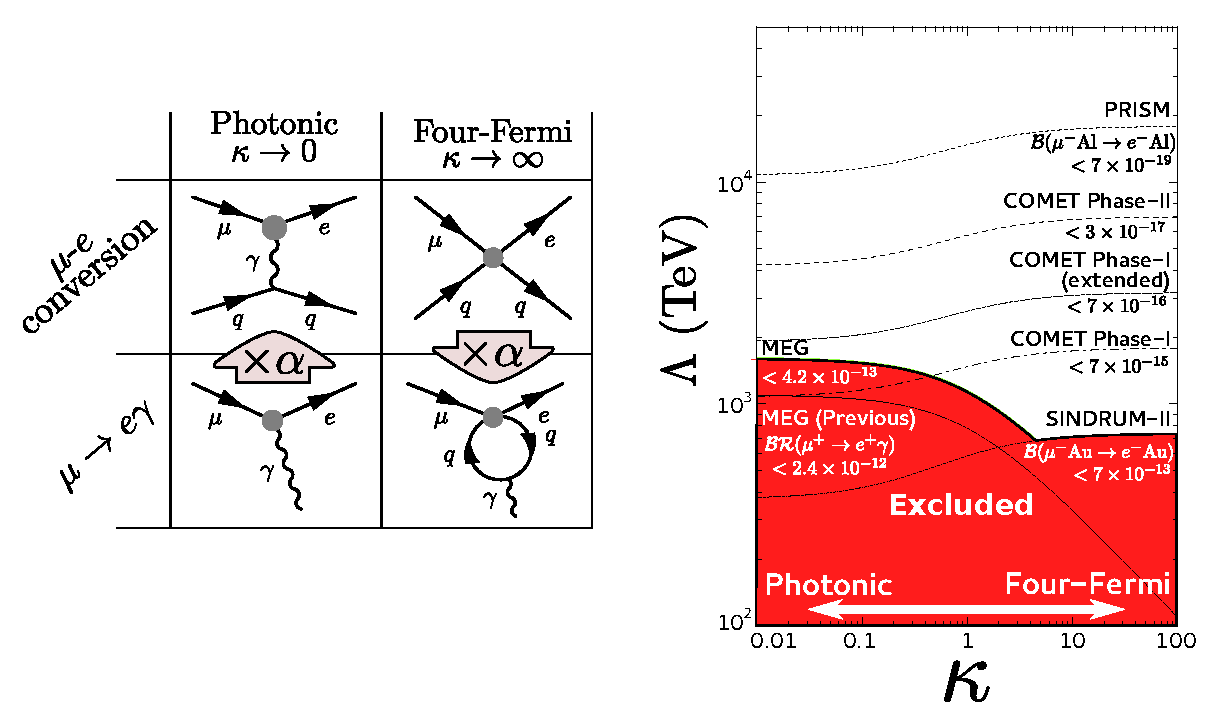
\includegraphics[width=0.85\textwidth]{figs/theory/MuecVsMueg.pdf}
%}
\caption{\figlabel{theory:muecVsMueg}
Searches for \mueconv and \muegamma have relative sensitivities that depend on the underlying physics, making the two channels highly complementary.
As shown on the left, New Physics can produce a signal in both channels, but one channel or the other can be comparatively suppressed due to the need to include extra vertices and loops.
The plot on the right is adapted from~\cite{ProposalPhase1}, based on~\cite{DEGOUVEA2009303}, and shows the relative sensitivity for the toy lagrangian of equation~\eq{theory:toy} as a function of $\kappa$, how non-photonic the New Physics is, and $\Lambda$, the mass scale assuming coupling strengths of unity.
}
%\footnote{though the author has failed to reproduce the stereoscopic effect with his own eyes}
\end{figure}
}

